\documentclass[sigconf]{acmart}
\AtBeginDocument{%
  \providecommand\BibTeX{{%
    Bib\TeX}}}

%% Rights management information.  This information is sent to you
%% when you complete the rights form.  These commands have SAMPLE
%% values in them; it is your responsibility as an author to replace
%% the commands and values with those provided to you when you
%% complete the rights form.
\setcopyright{acmcopyright}
\copyrightyear{tbd}
\acmYear{tbd}
\acmDOI{tbd}

%% These commands are for a PROCEEDINGS abstract or paper.
\acmConference[Conference acronym 'XX]{Make sure to enter the correct conference title from your rights confirmation emai}{tbd}{tbd}
%%
%%  Uncomment \acmBooktitle if the title of the proceedings is different
%%  from ``Proceedings of ...''!
%%
%%\acmBooktitle{Woodstock '18: ACM Symposium on Neural Gaze Detection,
%%  June 03--05, 2018, Woodstock, NY}
\acmPrice{15.00}
\acmISBN{tbd}


\usepackage{amsmath,amsfonts}
\usepackage{amsthm}
\usepackage{algorithm}
\usepackage{algpseudocode}
\usepackage{cleveref}
\usepackage{fancybox}
\usepackage{makecell}
\usepackage{arydshln}
\usepackage{subfigure}
    
%% New commands goes here
\newcommand{\Enote}[1]{\color{purple}Enote: #1\color{black}}
\newcommand{\Yaxin}[1]{\color{purple}Yaxin: #1\color{black}}

\newcommand{\Gen}{{\sf Gen}}
\newcommand{\Eval}{{\sf Eval}}
\newcommand{\FullEval}{{\sf FullEval}}
\newcommand{\Encode}{{\sf Encode}}
\newcommand{\Decode}{{\sf Decode}}
\newcommand{\row}{{\sf row}}
\newcommand{\seed}{{\sf seed}}
\newcommand{\sign}{{\sf sign}}
\newcommand{\map}{{\sf map}}
\newcommand{\stat}{{\sf stat}}
\newcommand{\poly}{{\sf poly}}

\newcommand{\OKVS}{{\sf OKVS}}
\newcommand{\Adv}{{\sf Adv}}
    
\newcommand{\GG}{\mathbb{G}}
\newcommand{\NN}{\mathbb{N}}
\newcommand{\ZZ}{\mathbb{Z}}
\newcommand{\FF}{\mathbb{F}}

\newcommand{\ipd}[2]{\langle #1, #2 \rangle}

\newtheorem{theorem}{Theorem}
\newtheorem{lemma}[theorem]{Lemma}
\newtheorem{claim}[theorem]{Claim}
\newtheorem{fact}[theorem]{Fact}
\newtheorem{definition}[theorem]{Definition}
\newtheorem{example}[theorem]{Example}
\newtheorem{remark}[theorem]{Remark}
\newtheorem{construction}{Construction}
\newtheorem{corollary}[theorem]{Corollary}
\newtheorem{proposition}[theorem]{Proposition}
%%
\begin{document}

%%
%% The "title" command has an optional parameter,
%% allowing the author to define a "short title" to be used in page headers.
\title{Notes for New Constructions of DMPF}

\author{tbd}
%\authornote{}
%\email{tbd}
%\affiliation{%
  %\institution{tbd}
  %\streetaddress{P.O. Box 1212}
  %\city{tbd}
  %\state{tbd}
  %\country{tbd}
  %\postcode{tbd}
%}

%%
%% By default, the full list of authors will be used in the page
%% headers. Often, this list is too long, and will overlap
%% other information printed in the page headers. This command allows
%% the author to define a more concise list
%% of authors' names for this purpose.
\renewcommand{\shortauthors}{tbd}

\begin{abstract}
  tbd. 
\end{abstract}

%%
%% The code below is generated by the tool at http://dl.acm.org/ccs.cfm.
\begin{CCSXML}
  <ccs2012>
     <concept>
         <concept_id>10003752.10003777.10003788</concept_id>
         <concept_desc>Theory of computation~Cryptographic primitives</concept_desc>
         <concept_significance>500</concept_significance>
         </concept>
   </ccs2012>
\end{CCSXML}
  
\ccsdesc[500]{Theory of computation~Cryptographic primitives}

%%
%% Keywords. The author(s) should pick words that accurately describe
%% the work being presented. Separate the keywords with commas.
\keywords{tbd}

%\received{20 February 2007}
%\received[revised]{12 March 2009}
%\received[accepted]{5 June 2009}

\maketitle

\section{Introduction}
tbd

\section{Preliminary}
  \section{Preliminary}

\subsection{Basic Notations}



 \paragraph{Point and multi-point functions.} Given a domain size $N$ and Abelian group $\GG$, a \emph{point function} $f_{\alpha,\beta}:[N]\rightarrow\GG$ for $\alpha\in[N]$ and $\beta\in\GG$ evaluates to $\beta$ on input $\alpha$ and to $0\in\GG$ on all other inputs. We denote by $\hat{f}_{\alpha,\beta}=(N,\hat{\GG},\alpha,\beta)$ the representation of such a point function. A \emph{$t$-point function} $f_{A,B}:[N]\rightarrow \GG$ for $A=(\alpha_1,\cdots\alpha_t)\in[N]^t$ and $B=(\beta_1,\cdots,\beta_t)\in \GG^t$ evaluates to $\beta_i$ on input $\alpha_i$ for $1\le i\le t$ and to $0$ on all other inputs. Denote $\hat{f}_{A,B}(N,\hat{\GG},t,A,B)$ the representation of such a $t$-point function. Call the collection of all $t$-point functions for all $t$ \emph{multi-point functions}. 
 
\Enote{MPF. Also representation of groups.}
 
\subsection{Distributed Multi-Point Functions}

\Enote{should directly adapt to multi-point function case}

We begin by defining a slightly generalized notion of distributed point functions (DPFs), which accounts for the extra parameter $\GG'$. \Yaxin{What is $\GG'$?}

%\yuval{Made some small stylistic changes below (similar changes may apply elsewhere). Should citations to GI14,BGI16. }
\begin{definition}[DPF \cite{EC:GilIsh14,CCS:BoyGilIsh16}]\label{def:dpf}
A 
%$t$-private $m$-server 
(2-party)
\emph{distributed point function (DPF)}
%, or $(m,t)$-DPF for short, 
is a triple of algorithms %$\Pi=(\Gen,\Eval_0,\ldots,\Eval_{m-1})$ 
$\Pi=(\Gen,\Eval_0,\Eval_1)$
with the following syntax: 
\begin{itemize}
    \item $\Gen(1^\lambda,\hat{f}_{\alpha,\beta})\rightarrow (k_0,k_1)$: On input security parameter $\lambda\in\NN$ and point function description $\hat{f}_{\alpha,\beta}=(N,\hat{\GG},\alpha,\beta)$, the (randomized) key generation algorithm $\Gen$ returns a pair of keys $k_0,k_1\in\{0,1\}^*$. \Yaxin{Matan points out: we want efficient procedures, i.e., $|k_b|\in\poly(\lambda)$. Stress it here or add efficiency requirement?} 
    We assume that $N$ and $\GG$ are determined by each key.
    \item $\Eval_b(k_b,x)\rightarrow y_b$: On input key $k_b\in\{0,1\}^*$ and input $x\in[N]$ the (deterministic) evaluation algorithm of server $b$, $\Eval_b$ returns 
    %a group element 
    $y_b\in\GG$.
\end{itemize}
%The algorithms $\Pi=(\Gen,\Eval_0,\ldots,\Eval_{m-1})$ should 
We require $\Pi$ to satisfy the following requirements:
\begin{itemize}
    \item \textbf{Correctness:} For every $\lambda$, $\hat{f}=\hat{f}_{\alpha,\beta}=(N,\hat{\GG},\alpha,\beta)$ such that $\beta\in\GG$, and $x\in[N]$, for $b=0,1$,  
    $$\Pr\left[(k_0,k_1)\leftarrow\Gen(1^\lambda,\hat{f}), \sum_{i=0}^{1}\Eval_b(k_b,x)=f_{\alpha,\beta}(x)\right]=1$$
    \item \textbf{Security:} Consider the following semantic security challenge experiment for corrupted server $b\in\{0,1\}$:
    \begin{enumerate}
        \item The adversary produces two point function descriptions $(\hat{f}^0=(N,\hat\GG,\alpha_0,\beta_0),\hat{f}^1=(N,\hat\GG,\alpha_1,\beta_1))\leftarrow\mathcal{A}(1^\lambda)$, where $\alpha_b\in[N]$ and $\beta_b\in\GG$.
        \item The challenger samples $b\gets\{0,1\}$ and $(k_0,k_1)\leftarrow\Gen(1^\lambda,\hat{f}^b)$.
        \item The adversary outputs a guess $b'\leftarrow\mathcal{A}(k_b)$.
    \end{enumerate}
    Denote by $\Adv(1^\lambda,\mathcal{A},i)=\Pr[b=b']-1/2$ the advantage of $\mathcal{A}$ in guessing $b$ in the above experiment. For every non-uniform polynomial time adversary $\mathcal{A}$ there exists a negligible function $\nu$ such that $\Adv(1^\lambda,\mathcal{A},i) \le \nu(\lambda)$ for all $\lambda \in \NN$.
%    For circuit size bound $S=S(\lambda)$ and advantage bound $\epsilon(\lambda)$, we say that $\Pi$ is $(S,\epsilon)$-secure if for all $i\in\{0,1\}$ and all non-uniform adversaries $\mathcal{A}$ of size $S(\lambda)$ and sufficiently large $\lambda$, we have $\Adv(1^\lambda,\mathcal{A},i)\leq\epsilon(\lambda)$. We say that $\Pi$ is:
%    \begin{itemize}
%        \item \emph{Computationally $\epsilon$-secure} if it is $(S,\epsilon)$-secure for all polynomials $S$.
%        \item \emph{Computationally secure} if it is $(S,1/S)$-secure for all polynomials $S$.
%        %\item \emph{Statistically $\epsilon$-secure} if it is $(S,\epsilon)$-secure for all $S$.
%        %\item \emph{Perfectly secure} if it is statistically $0$-secure.
%    \end{itemize}
\end{itemize}
%If the security threshold $t$ is unspecified, we assume it is $t=1$.
\end{definition}

\begin{definition}[DMPF]\label{def:dmpf}
  A 
  %$t$-private $m$-server 
  (2-party)
  \emph{distributed multi-point function (DMPF)}
  %, or $(m,t)$-DPF for short, 
  is a triple of algorithms %$\Pi=(\Gen,\Eval_0,\ldots,\Eval_{m-1})$ 
  $\Pi=(\Gen,\Eval_0,\Eval_1)$
  with the following syntax: 
  \begin{itemize}
      \item $\Gen(1^\lambda,\hat{f}_{A,B})\rightarrow (k_0,k_1)$: On input security parameter $\lambda\in\NN$ and point function description $\hat{f}_{A,B}=(N,\hat{\GG},t,A,B)$, the (randomized) key generation algorithm $\Gen$ returns a pair of keys $k_0,k_1\in\{0,1\}^*$. \Yaxin{On Matan's behalf: same comment as well. Maybe $|k_i|=\poly(\lambda,t)$. }
      \item $\Eval_b(1^\lambda, k_b,x)\rightarrow y_b$: On input key $k_b\in\{0,1\}^*$ and input $x\in[N]$ the (deterministic) evaluation algorithm of server $b$, $\Eval_b$ returns $y_b\in\GG$.
  \end{itemize}
  We require $\Pi$ to satisfy the following requirements:
  \begin{itemize}
      \item \textbf{Correctness:} For every $\lambda$, $\hat{f}=\hat{f}_{A,B}=(N,\hat{\GG},t,A,B)$ such that $B\in\GG^t$, and $x\in[N]$, for $b=0,1$,
      $$\Pr\left[(k_0,k_1)\leftarrow\Gen(1^\lambda,\hat{f}), \sum_{i=0}^{1}\Eval_b(k_b,x)=f_{A,B}(x)\right]=1$$
      \item \textbf{Security:} Consider the following semantic security challenge experiment for corrupted server $b\in\{0,1\}$:
      \begin{enumerate}
          \item The adversary produces two $t$-point function descriptions $(\hat{f}^0=(N,\hat\GG,t,A_0,B_0),\hat{f}^1=(N,\hat\GG,t,A_1,B_1))\leftarrow\mathcal{A}(1^\lambda)$, where $\alpha_b\in[N]$ and $\beta_b\in\GG$.
          \item The challenger samples $b\gets\{0,1\}$ and $(k_0,k_1)\leftarrow\Gen(1^\lambda,\hat{f}^b)$.
          \item The adversary outputs a guess $b'\leftarrow\mathcal{A}(k_b)$.
      \end{enumerate}
      Denote by $\Adv(1^\lambda,\mathcal{A},i)=\Pr[b=b']-1/2$ the advantage of $\mathcal{A}$ in guessing $b$ in the above experiment. For every non-uniform polynomial time adversary $\mathcal{A}$ there exists a negligible function $\nu$ such that $\Adv(1^\lambda,\mathcal{A},i) \le \nu(\lambda)$ for all $\lambda \in \NN$.
  \end{itemize}
  \end{definition}
 
 We will also be interested in applying the evaluation algorithm on \emph{all} inputs. Given a DMPF $(\Gen,\Eval_0,\Eval_1)$, we denote by $\FullEval_b$ an algorithm which computes $\Eval_b$ on every input $x$. Hence, $\FullEval_b$ receives only a key $k_b$ as input.

 One can construct a DMPF scheme for $t$-point functions by simply summing $t$ DPFs. We denote this DMPF scheme as the na\"ive construction. 
\begin{construction}[Na\"ive construction of DMPF]
  Given DPF for domain of size $N$ and output group $\GG$, we can construct a DMPF scheme for $t$-point functions with domain size $N$ and output group $\GG$ as follows: 
  \begin{itemize}
    \item $\Gen(1^\lambda, \hat{f}_{A, B})\rightarrow (k_0, k_1)$: Suppose $A = \{\alpha_1,\dots, \alpha_t\}$ and $B = \{\beta_1,\dots, \beta_t\}$. For $1\le i\le t$, invoke DPF$.\Gen(1^\lambda, \hat{f}_{\alpha_i, \beta_i})\rightarrow (k_0^i, k_1^i)$. Set $(k_0, k_1) = (\{k_0^i\}_{i\in [t]}, \{k_1^i\}_{i\in [t]})$. 
    \item $\Eval_b(k_b, x)\rightarrow y_b$: Compute $y_b = \sum_{i\in [t]}$DPF$.\Eval_b(k_b^i, x)$. 
    \item $\FullEval_b(k_b)\rightarrow Y_b$: Compute $Y_b = \sum_{i\in [t]}$DPF$.\FullEval_b(k_b^i, x)$. 
  \end{itemize}
\end{construction}
When the DPF scheme is correct and secure, the na\"ive construction of DMPF is also correct and secure. We note that the keysize and running time of $\Gen$, $\Eval$ and $\FullEval$ of the na\"ive construction of DMPF equals $t\times $ the keysize and $t\times$ the running time of $\Gen$, $\Eval$ and $\FullEval$ of DPF, respectively. We aim to provide DMPF schemes that has $\Eval$ and $\FullEval$ time almost independent to $t$. 
 
 

\subsection{Batch Code}
We introduce probabilistic batch code, a batch code permitting small decoding errors, which can be used to construct DMPF (see \cref{con:DMPF_batch_code}). 
\begin{definition}[Probabilistic Batch Code (PBC)\cite{cryptoeprint:2017/1142,10.1145/1007352.1007396,yeo_cuckoo_2023}]
  An $(N,M,t,m,b,\epsilon)$-PBC over alphabet $\Sigma$ is given by a tuple of efficient algorithms $(\Encode,\Schedule,\Decode)$ with public randomness $r$ such that:
  \begin{itemize}
    \item $\Encode_r(x\in\Sigma^N)\rightarrow (C_1,C_2,\dots,C_m)$: Any string $x\in\Sigma^N$ is encoded into an $m$-tuple of codewords $C_1,C_2,\cdots C_m\in\Sigma^*$ of total length $M$.
    \item $\Schedule_r(I)\rightarrow (S_1,S_2,\dots, S_m)$: For any $I\subseteq [N]$ and $|I|\le t$, $\Schedule_r$ outputs $m$ sets of indices to read in the $m$ codewords, respectively, and that for all $i$, $|S_i|\le b$. 
    \item $\Decode_r(I,C_1|_{S_1},C_2|_{S_2},\dots,C_m|_{S_m})\rightarrow x|_I$: On input a set $I\subseteq[N]$ of $\le t$ distinct indices in $[N]$, and the scheduled indices to read in the $m$ codewords, recover the subset of $x$ indexed by $I$. 
    \item Correctness: for any string $x$ and any set $I$ of $t$ distinct indices in $[N]$, 
    \[
    \begin{split}
      \Pr_r[&(C_1,\dots, C_m)\gets \Encode_r(x), \\
      &(S_1,\dots ,S_m)\gets \Schedule_r(I), \\
      &x_I\not= \Decode_r(I,C_1|_{S_1},\dots,C_m|_{S_m} )] \le \epsilon
    \end{split}
    \]
  \end{itemize}
\end{definition}

We will focus on the case $b=1$ and a special class of batch code called combinatorial batch code (CBC)\cite{cryptoeprint:2017/1142,10.1145/1007352.1007396,cryptoeprint:2008/306}, where each codeword $C_i$ is a subset of $x$ and the decoding algorithm recovers $x|_I$ by collecting from the scheduled sets of indices. 
In this case, the encoding algorithm is equivalent to replicating and allocating the indices in $[N]$ to $m$ buckets (codewords), and the scheduling algorithm is equivalent to finding a prefect matching from the size-$t$ subset $I\subseteq[N]$ to the $m$ buckets, while indicating which position in each bucket should be read. 

\Yaxin{Add example instantiation (random regular bipartite graph) and explain it is not efficient?  }

Based on the definition of CBC, a probabilistic CBC (PCBC) is a CBC with failure probability when decoding. We mention Cuckoo hashing algorithm\cite{10.1007/3-540-44676-1_10} as a concrete instantiation of PCBC\cite{cryptoeprint:2017/1142,yeo_cuckoo_2023}.

\paragraph{$w$-way cuckoo hashing.}Given $t$ balls, $m=et$ buckets ($e$ is some expansion parameter that is bigger than 1), and $w$ independent hash functions $h_1, h_2,\cdots, h_w$ randomly mapping every ball to a bucket, allocates all balls to the buckets such that each bucket contains at most one ball through the following process: 
\begin{itemize}
  \item[1.] Choose an arbitrary unallocated ball $b$. If there is no unallocated ball, output the allocation. 
  \item[2.] Choose a random hash function $h_i$ compute the bucket index $h_i(b)$. If this bucket is empty, then allocate $b$ to this bucket and go to step 1. If this bucket is not empty and filled with ball $b'$, then evict $b'$, allocate $b$ to this bucket, set $b'$ the current unallocated ball, and repeat step 2. 
\end{itemize}
If the algorithm terminates then its output is an allocation of balls to buckets such that each bucket contains at most one ball. However there is no guarantee that the algorithm will terminate - it may end up in a loop and keeps running forever. To fixed this problem, the algorithm should be given a fixed amount of time to run, or equipped with a loop detection process to guarantee termination. We call it a \emph{failure} whenver the algorithm fails to output a proper allocation where each bucket contains at most one ball. 

\paragraph{The failure probability of cuckoo hashing.}Let's denote the failure probability of $w$-way cuckoo hashing to be $\epsilon=2^{-\lambda_{\stat}}$. In practice we usually consider the statistical security parameter $\lambda_{\stat}$ to be $40$. The relations among the number of balls $t$, the number of hash functions $w$, the number of buckets $m$ and the security parameters $\lambda_\stat$ are listed in \Cref{tab:cuckoo_hashing_prm}. 

\begin{table*}
  \renewcommand\arraystretch{1.5}
  %\scalebox{1}{
  \begin{threeparttable}
  \caption{he relations among the number of balls $t$, the number of hash functions $w$, the number of buckets $m$ and the security parameters $\lambda_\stat$ in cuckoo hashing. }
  \label{tab:cuckoo_hashing_prm}
    \begin{tabular}{cccccc}
      \toprule 
      %Header
      &  Type&$t$ &$\lambda_\stat$ & $w$ & $e = m/t$  \\
       

      \midrule
      \cite[Theorem 1]{yeo_cuckoo_2023}\tnote{$\dag$}& Asymptotic & & & $O(\sqrt{\lambda_{\stat}\log t})$ & $O(1)$ \\
     
      \cline{1-6}
      \cite{cryptoeprint:2021/580}& Asymptotic & & & 3 & $O(\lambda_\stat+\log t)$ \\

      \cline{1-6}
      \cite[Appendix B]{cryptoeprint:2018/579} & Empirical & $t\ge 4$ & \makecell{$\lambda_\stat = a_t\cdot e - b_t - \log t$\\$a_t = 123.5\cdot {\sf CDF_{Normal}}(x=t, \mu = 6.3, \sigma = 2.3)$\\$b_t = 120\cdot {\sf CDF_{Normal}}(x=t, \mu = 6.45, \sigma = 2.18)$} & 3\tnote{$\ddag$} & $e$ \\

      \cline{1-6}
      \makecell{\cite{cryptoeprint:2021/580}\\ simplifying the above} & Empirical & $t\ge 30$\tnote{*} & \makecell{$\lambda_\stat = 123.5 e -120 - \log t$} & 3 & $e$\\

      \cline{1-6}
      \multirow{2}{*}{\cite{chen_fast_2017}\tnote{**}} &\multirow{2}{*}{ Empirical }& $11041$ & $40\,(\lambda_\stat = 124.4 e - 144.6)$ & 3 &$m=2^{14},\,e\approx 1.5$\\
      \cline{3-6}
      & & $5535$ & $40\,(\lambda_\stat = 125 e - 145)$ & 3 &$m=2^{13}, \, e\approx 1.5$\\
      
      \bottomrule
    \end{tabular}	
    \begin{tablenotes}
      \item [$\dag$] $O(\sqrt{\lambda_\stat \log t})$ queries to the hash functions and supposes the hash functions from a $O(t\sqrt{\lambda_\stat \log t})$-wise independent hash function family. 
      \item [$\ddag$] Parameters are only slightly different for $w>3$. 
      \item [*] Should extend to smaller $t$ like $t = 16, 25$.
      \item [**]It first fixes $m = 2^{13}, 2^{14}$ and then computes the correlation between $\lambda_\stat$ and $e$.   
      \end{tablenotes}
  \end{threeparttable}
  %}
\end{table*}

%However we use cuckoo hashing to construct DMPF for $t$-point functions, in which case we'd also care about $t$ being small, say $2,3$ or $100$, and $m$ should not be too large. In this sense the previous empirical results are not complete. 

With the $t$ balls replicated and allocated to $m$ buckets, the cuckoo hashing algorithm essentially finds a perfect matching from $t$ balls to $m$ buckets, which coincides with the form of (probabilistic) CBC decoding. Therefore a PCBC follows directly from a cuckoo hashing scheme: \Yaxin{Dec 31: The following construction is mentioned in \cite{yeo_cuckoo_2023}. There are several points to note: 

(1) \cite{yeo_cuckoo_2023} modified the hash functions' domain in the following way: it divides the $m$ buckets evenly to $w$ blocks, and for $1\le i\le w$, $h_i:[N]\rightarrow [m/w]$ maps an element to a bucket in the $i$th block. The paper does this to claim better asymptotic provable success probability of cuckoo hashing, but using superconstant number ($w = \lambda_\stat/\log\log N$) of hash functions, which does not align with empirical results that suggests constant number (say 3) of hash functions. I think to us this means that if making $h_i$ to map to the $i$th block could be useful in implementation somehow (although I doubt this), then it also makes sense to do this modification. 

(2) It should be mentioned that both the capacity of cuckoo-hashing bins (which is 1 here) and the number of lookup in each $C_i$ that PCBC is allowed (also 1 here) can be simultaneously generalized to any number $l$ along with different parameters and overheads, but the paper still applied only $l=1$ case to applications like batch PIR, and I haven't seen any efficient empirical parameters and results for $l>1$ setting. However it is plausible to use general $l$ along with $O(t/l)$ buckets, each expanded to a $\DMPF_l$ truth table. It may be mentioned as a future direction in the end. }

\begin{construction}[PCBC from cuckoo hashing]
  Given $w$-way cuckoo hashing as a sub-procedure allocating $t$ balls to $m$ buckets with failure probability $\epsilon$, an $(N,wN,t,m,\epsilon)$-PCBC is as follows: 
  \begin{itemize}
    \item $\Encode_r(x\in\Sigma^N)\rightarrow (C_1,\cdots,C_m)$: Use $r$ to determine $w$ independent random hash functions $h_1,h_2,\cdots h_w$ that maps from $[N]$ to $[m]$.  Let $C_j$ be $\{x[i]:h_l(i) = j$ for some $l\in [w]\}$, in ascending order of $i$. 
    \item $\Decode_r(I, C_1,\cdots, C_m)\rightarrow \{x[i]\}_{i\in I}$: Determine $h_1,\cdots, h_w$ as in $\Encode$. For $I$ of size $t$, find a perfect matching from $I$ to $[m]$ using a $w$-way cuckoo hashing scheme. For each $i\in I$, fetch $x[i]$ from $C_j$ where $i$ and $j$ are matched in the perfect matching. Note that $x[i]$ can be found in the $k$th position of $C_j$ where $i$ is the $k$th smallest index of $\{i:h_l(i) = j$ for some $l\in [w]\}$. 
  \end{itemize}
\end{construction}
%The above PCBC scheme has its encoding and decoding process independent of the content of the input string $x$. 
An ambiguous point in $\Decode_r$ is how to find the index of $x[i]$ in $C_j$ it is mapped to. We  display two solutions to this index finding problem: 
\begin{enumerate}
  \item When $N$ is a feasible number, one can directly compute the entire hash tables derived by $h_1,\dots, h_w$ and compute the index of $x[i]$ in $C_j$. 
  \item One can implement $w$ hash functions by a single \emph{random permutation} $P$ mapping from $[w]\times [N]$ to $[m]\times [B]$, where $B = wN/m$. Invocation of $h_i(j)$ is done by computing $P(i,j)$, which outputs the bucket number in $[m]$ and the index in $[B]$. Note that in this case $h_1,\dots,h_w$ are not independent random hash functions, but as long as they \Yaxin{satisfy some sufficient independence property. To be clarified. }This solution is noted in \cite{cryptoeprint:2021/580} where $P$ is realized by a PRP. 
\end{enumerate}
\subsection{DMPF Construction from CBC}
We display the construction of DMPF from black-box usage of DPF basing on PCBC with appropriate parameters, which has been discussed in previous literature\cite{cryptoeprint:2019/273,cryptoeprint:2021/580}. As discussed before, we assume that the PCBC encoding and decoding are oblivious of the content of the input string.  
\begin{construction}[DMPF from DPF basing on PCBC]\label{con:DMPF_batch_code}
  Given DPF for any domain of size no larger than $N$ and output group $\GG$, and an $(N,M,t,m,\epsilon)$-PCBC with alphabet $\Sigma=\GG$, we can construct a DMPF scheme for $t$-point functions with domain size $N$ and output group $\GG$ as follows: 
  \begin{itemize}
    \item $\Gen(1^\lambda, \hat{f}_{A,B})\rightarrow (k_0,k_1)$: Suppose $A=\{\alpha_1,\cdots,\alpha_t\}$ and $B=\{\beta_1,\cdots,\beta_t\}$. Compute $\Encode([N])\rightarrow (C_1,\cdots,C_m)$ according to the PCBC. Then run $\Decode(A, C_1,\cdots, C_m)$ to determine a perfect matching from $A$ to $\{C_1,\cdots,C_m\}$. For $1\le i\le m$, let $f_i:[|C_i|]\rightarrow \GG$ be the following: 
    \begin{itemize}
      \item If $C_i$ is assigned none of $A$ by the perfect matching, then set $f_i$ to be the all-zero function. 
      \item If exactly one $\alpha_j$ of $A$ is assigned to the $l$th position of $C_i$, then set $f_i$ to be the point function that outputs $\beta_j$ on $l$ and 0 elsewhere. 
    \end{itemize}
    For $1\le i\le m$, invoke DPF$.\Gen(1^\lambda, f_i)\rightarrow (k_0^i,k_1^i)$. Set $(k_0,k_1)=(\{k_0^i\}_{i\in [m]}, \{k_1^i\}_{i\in [m]})$. If $\Decode$ fails then run $\Encode$ and $\Decode$ again with fresh randomness. 
    \item $\Eval_b(k_b,x)\rightarrow y_b$: Follow $\Encode([N])$ to determine the positions $l_{j_1},l_{j_2},\cdots, l_{j_s}$ such that the $x$ is sent to the $l_{j_i}$-th position of $C_{j_i}$ (since the allocation of indices is oblivious of the content of $TT$). Compute $y_b=\sum_{i=1}^s$DPF$.\Eval_b(k_b^{j_i},l_i)$. 
    \item $\FullEval_b(k_b)\rightarrow Y_b$: Compute $Y_b^i = $DPF$.\FullEval_b(k_b^i)$ for $1\le i\le m$. For each input $x\in [N]$, follow $\Encode([N]])$ to choose a position $l_x$ in bucket $C_{j_x}$ that $x$ is sent to. Let $Y_b[x]\gets Y_b^{j_x}[l_x]$. 
  \end{itemize}
The scheme is correct with overwhelming probability and has distinguish advantage $<2\epsilon$. 
\end{construction}
Note that if one use CBC instead of PCBC then the DMPF scheme is perfectly correct and secure. 

When instantiating PCBC using $w$-way cuckoo hashing, the \emph{key generation time} is roughly the time for computing cuckoo hashing algorithm, the time for finding $t$ indices for $t$ elements in the buckets, plus the total time of all DPF$.\Gen(1^\lambda, f_i)$. The \emph{evaluation time} is roughly the time for finding $w$ indices for one element in the buckets plus the total time of all DPF$.\Eval_b(k_b^{j_i},l_i)$. Similarly, the \emph{full-domain evaluation time} is roughly the time for finding $N$ indices for $N$ elements in the buckets plus the total time of all DPF$.\FullEval_b(k_b^{j})$ for $j=1,\dots,m$. 

\subsection{Oblivious Key-Value Stores}\label{sec:prelim_okvs}
We introduce the notion of Oblivious key-value stores (OKVS) which can be used to construct DMPF. OKVS was originally proposed as a primitive for private set intersection (PSI) protocols (see \cite{cryptoeprint:2021/883,cryptoeprint:2022/320}). 
\begin{definition}[Oblivious Key-Value Stores (OKVS)\cite{cryptoeprint:2021/883,cryptoeprint:2022/320}]\label{def:OKVS}
  An Oblivious Key-Value Stores scheme is a pair of randomized algorithms $(\Encode_r,\Decode_r)$ with respect to a statistical security parameter $\lambda_{\sf stat}$ and a computational security parameter $\lambda$, a randomness space $\{0,1\}^\kappa$, a key space $\mathcal{K}$, a value space $\mathcal{V}$, input length $t$ and output length $m$. The algorithms are of the following syntax: 
  \begin{itemize}
    \item $\Encode_r(\{(k_1,v_1),(k_2,v_2),\cdots,(k_t,v_t)\})\rightarrow P$: On input $t$ key-value pairs with distinct keys, the encode algorithm with randomness $r$ in the randomness space outputs an encoding $P\in\mathcal{V}^m\cup\bot$.
    \item $\Decode_r(P,k)\rightarrow v$: On input an encoding from $\mathcal{V}^m$ and a key $k\in\mathcal{K}$, output a value $v$. 
  \end{itemize}
  We require the scheme to satisfy
  \begin{itemize}
    \item For all $S\in(\mathcal{K}\times\mathcal{V})^t$, $\Pr_{r\leftarrow\{0,1\}^\kappa}[\Encode_r(S)=\bot]\le 2^{-\lambda_{\sf stat}}$. 
    \item For all $S\in(\mathcal{K}\times \mathcal{V})^t$ and $r\in \{0,1\}^\kappa$ such that $\Encode_r(S)\rightarrow P\not=\bot$, it is the case that $\Decode_r(P,k)\rightarrow v$ whenever $(k,v)\in S$. 
    \item \textbf{Obliviousness: }Given any distinct key sets $\{k_1^0,k_2^0,\cdots,k_t^0\}$ and $\{k_1^1,k_2^1,\cdots,k_t^1\}$ that are different, if they are paired with random values then their encodings are computationally indistinguishable, i.e., 
  \begin{align*}
    &\{r, \Encode_r(\{(k_1^0,v_1),\cdots,(k_t^0,v_t)\})\}_{v_1,\cdots,v_t\leftarrow \mathcal{V},r\leftarrow\{0,1\}^\kappa}\\
    \approx_c &\{r, \Encode_r(\{(k_1^1,v_1),\cdots,(k_t^1,v_t)\})\}_{v_1,\cdots,v_t\leftarrow \mathcal{V},r\leftarrow\{0,1\}^\kappa}
  \end{align*}
  \end{itemize}
One can obtain a \emph{linear OKVS} if in addition require:
\begin{itemize}
  \item \textbf{Linearity: }There exists a function family $\{\row_r:\mathcal{K}\rightarrow\mathcal{V}^m\}_{r\in\{0,1\}^\kappa}$ such that $\Decode_r(P,k) = \ipd{\row_r(k)}{P}$. 
\end{itemize}
\end{definition}
The $\Encode$ process for a linear OKVS is the process of sampling a random $P$ from the set of solutions of the linear system $\{\ipd{\row_r(k_i)}{P} = v_i\}_{1\le i\le t}$. 

We evaluate an OKVS scheme by its rate ($\frac{\text{input length }t}{\text{output length }m}$), encoding time and decoding time. 

The most na\"ive OKVS construction is encoding $S = \{(k_i, v_i)\}_{1\le i\le t}$ to a random truth table $TT:\mathcal{K}\rightarrow \mathcal{V}$ such that $TT(k_i) = v_i$ for all $1\le i\le t$. Note that to ensure obliviousness, for $k$ not appearing in $S$, the encoding should set $TT(k)$ to a random value. However this na\"ive construction is very inefficient since it requires the encoding size to be $m=|\mathcal{K}|$, and hence its rate $\frac{t}{|\mathcal{K}|}$ can be tiny. 

A well-known, optimal-rate OKVS construction is encoding $t$ key-value pairs using a deg-$t$ polynomial: 
\begin{construction}[Polynomial]\label{con:OKVS_polynomial}
  Suppose $\mathcal{K} = \mathcal{V}=\FF$ is a field. Set 
  \begin{itemize}
    \item $\Encode(\{(k_i,v_i)\}_{1\le i\le t}) \rightarrow P$ where $P$ is the coeffients of a $(t-1)$-degree $\FF$-polynomial $g_P$ that $g_P(k_i) = v_i$ for $1\le i\le t$. 
    \item $\Decode(P,k)\rightarrow g_P(k)$. 
  \end{itemize}
\end{construction}
The polynomial OKVS possesses an optimal encoding size $m=n$, but the $\Encode$ process is a polynomial interpolation which is only known to be achieved in time $O(t\log^2t)$. The time for a single decoding is $O(t)$ and that for batched decodings is (amortized) $O(\log^2 t)$. 

In the sequel we stress two alternative (linear) OKVS constructions that has near optimal encoding size but much better running time. 

\begin{construction}[RR22\cite{cryptoeprint:2021/883,cryptoeprint:2022/320}]\label{con:OKVS_sparse_matrix}
  Suppose $\mathcal{V}=\FF$ is a field. Set $\row_r(k):=\row_r^{\sf sparse}(k)||\row_r^{\sf dense}(k)$ where $\row_r^{\sf sparse}(k)$ outputs a uniformly random weight-$w$ vector in $\{0,1\}^{m_1}$, and $\row_r^{\sf dense}(k)$ outputs a short dense vector in $\FF^{m_2}$. 
  \begin{itemize}
    \item $\Encode_r(\{(k_i,v_i)\}_{1\le i\le t}) \rightarrow P$ where $P$ is randomly chosen from the solutions of the system $\{\ipd{\row_r(k_i)}{P} = v_i\}_{1\le i\le t}$, solved by the triangulation algorithm in \cite{cryptoeprint:2022/320}. If the system has no solution then output $\bot$. 
    \item $\Decode_r(P,k)\rightarrow \ipd{\row_r(k)}{P}$. 
  \end{itemize}
  We denote $m_1=et$, where $e$ is an expansion parameter indicating the rough blowup to store $t$ pairs. In practice the number of dense columns $m_2$ is usually set to a small constant. 
\end{construction}
This OKVS construction features an efficient encoding process, constant decoding time ($(w+m_2)$ additions and $m_2$ multiplications in $\FF$) while having a linear encoding size. 

$\Encode$ may output $\bot$ if the matrix formed by $\{\row_r(k_i)\}_{1\le i\le t}$ is not full-rank. Therefore we need to adjust the parameters $m_1=et$ and $m_2$ to ensure negligible error probability (represented by the statistical security parameter $\lambda_\stat$). The expansion parameter $e$ and the number of dense columns $m_2:=\hat{g}$ (where $\hat{g}$ is a parameter relating to the equation system solving process) are given by the analysis in \cite{cryptoeprint:2022/320}, with the range of $N$ from $2^6$ to $2^{18}$: Given $w$, $t$ and $\lambda_\stat$, the choices of the $e$ and $\hat{g}$ are fixed through the following steps: 
\begin{itemize}
  \item Set $e^* = \begin{cases}
    1.223 & w=3\\
    1.293 & w=4\\
    0.1485w+0.6845 & w\ge 5
  \end{cases}$.
  \item Compute $\alpha:=0.55 \log_2 t + 0.093w^3-1.01w^2 + 2.92w-0.13$.
  \item $e:=e^*+ 2^{-\alpha}(\lambda_\stat+9.2)$. 
  \item $\hat{g}:=\frac{\lambda_\stat}{(w-2)\log_2(et)}$. 
\end{itemize}


\Yaxin{Fix $t$ and $\lambda_\stat$, we want to find the best choice of $w$. The adavantageous choices of $w$ in \cite{cryptoeprint:2022/320} are $w=3$ and $w=5$. From the first sight when $w$ is smaller $e$ can be smaller but $\hat{g}$ will be larger. Since $w+\hat{g}$ stands for number of $\FF$-ADD's and $\hat{g}$ stands for number of $\FF$-MULT's in decoding, previously I thought $\hat{g}$ is the dominating factor of $\Decode$ running time. However table 1 in \cite{cryptoeprint:2022/320} suggests that $w=3$ outruns nearly all of other choices of $w$ while $w=5$ is almost 3 times slower in decoding time. This may suggest there are some other heavy computations other than $\FF$-MULT that need to be considered when evaluating running time. 

The range of $t$ previous literature \cite{cryptoeprint:2021/883,cryptoeprint:2022/320} have considered in their empirical results are also limited, which will be one of our problems. We want to cover small $t$, say $t<100$, while previous literature aiming for constructing PSI protocols usually consider very large $t$. }

One may let $row_r^{\sf dense}$ output a short dense vector in $\{0,1\}^{m_2}$ to avoid multiplication of large field elements in the encoding and decoding processes. To achieve same level of security one could simply set $m_2=\hat{g}+\lambda_\stat$, as proposed in \cite{cryptoeprint:2021/883,cryptoeprint:2022/320}. As indicated by the empirical results in \cite{cryptoeprint:2022/320}, this binary scheme is usually not as efficient as the original design. Therefore we mostly refer to \cref{con:OKVS_sparse_matrix}. 

\begin{construction}[RB-OKVS\cite{cryptoeprint:2023/903}]\label{con:OKVS_ribbon}
  Suppose $\mathcal{V} = \GG$ is a group. Let $\row_r(k)$ output a $\{0,1\}^m$ vector consisting of a width-$w$ random band. Formally speaking, $\row_r(k)$ first determine a starting point $1\le i\le m-w+1$ for the band, and then determine random $w$-bit string to fill in the positions $[i,i+w-1]$ of $\row_r(k)$ and leave the rest as 0 entries. 
  \begin{itemize}
    \item $\Encode_r(\{(k_i,v_i)\}_{1\le i\le t})\rightarrow P$ where $P$ is randomly chosen from the random band matrix system $\{\ipd{\row_r(k_i)}{P}=v_i\}_{1\le i\le t}$. If the system has no solution then output $\bot$. 
    \item $\Decode_r(P,k)\rightarrow \ipd{\row_r(k)}{P}$. 
  \end{itemize}
  Denote $m=et$ where $e>1$ is an expansion parameter indicating the blowup to store $t$ pairs. 
\end{construction}

The encoding time is equivalent to solving a random band matrix system, which can be efficiently done in $O(Nw+n\log n)$ time \cite{cryptoeprint:2023/903}. The decoding time is $w$ additions in $\FF$ and the rate can be very close to 1. 

Again, to guarantee the success of $\Encode$, the random band matrix must be full-rank with overwhelming probability. According to \cite{cryptoeprint:2023/903}, fixing $e>1$ and taking $w = O(\lambda_\stat/(e-1)+\log N)$ ensures the correctness and obliviousness with probability $2^{-\lambda_\stat}$ and $2^{-w}$, respectively. Practically, $e=1.03,1.05,1.07,1.1$ are taken while $w$ being several hundred to reach the security $\lambda_\stat=40$, with the choice of $N$ varying from $2^{10}$ to $2^{20}$. 

According to the comparison in \cite{cryptoeprint:2023/903} of the RR22-OKVS (\cref{con:OKVS_sparse_matrix}) and the RB-OKVS (\cref{con:OKVS_ribbon}) with the choices of $N = 2^{16}, 2^{20}, 2^{24}$, the RB-OKVS has a better rate and features a tradeoff between rate and encoding/decoding time (one can choose to have better rate with longer encoding/decoding time). The RB-OVS has better encoding time while the RR22-OKVS has better decoding time. 

\Yaxin{Maybe (and how to) put a (quantitative) summarizing table of OKVS efficiency here?}

\medskip

In our later sections, we will give the decoding efficiency of the OKVS the most priority. To this end, we refer to the RR22-OKVS (\cref{con:OKVS_sparse_matrix}) when instantiating OKVS. One may switch to other OKVS constructions depending on different needs in practice. 

\section{New DMPF constructions}
In this section, we display two new constructions of DMPF that follow the same paradigm shown in \cref{fig:DMPF_paradigm}. 

We begin by introducing the DMPF paradigm in \cref{fig:DMPF_paradigm}, which is based on the idea of the DPF construction in \cite{CCS:BoyGilIsh16}. Each key $k_b(b=0,1)$ generated by ${\sf Gen}(\hat{f}_{A,B})$ can span a height-$n$ ($n$ is the input length of $\hat{f}_{A,B}$) complete binary tree $T_b$ (call it the evaluation tree), with which party $b$ can evaluate the input $x=x_1\cdots x_n$ by starting from the root of this tree, on the $i$th layer going left if $x_i=0$ and going right if $x_i=1$, until reaching a leaf node then computing the result according to this leaf node. 

Each node of this tree is associated with a $\lambda$-bit seed and a $l$-bit sign. For a parent node on the $i$th layer with $\seed$ and $\sign$, its children's seeds and signs are generated by $\sf PRG(\seed)\oplus Correction$, where the $\sf Correction$ is determined by the parent node's position, its $\sign$ and a correction word $CW^{(i)}$ associated with that layer (computed by the method $\sf Correct()$). On a leaf node on the last layer, its $\seed$ will generate a random element in the output group, which will be corrected by adding a $\sf Correction$ determined by the leaf node's position, its sign and the last correction word $CW^{(n+1)}$ (computed by the method $\sf ConvCorrect()$). 

Call any path from the root a leaf corresponding to an input string in $A$ an accepting path. To force the correctness, we maintain the following invariance on the evaluation trees $T_0$, $T_1$ of the two parties: 
\begin{itemize}
  \item If a node is not on any accepting path, then $T_0$ and $T_1$ assign to it with the same seed and sign. 
  \item If a node is on an accepting path, then $T_0$ and $T_1$ assign to it with different signs that controls the corrections on its children (or on the output if the node is on the last layer). 
\end{itemize}

The paradigm contains four methods ($\sf GenCW$, $\sf GenConvCW$, $\sf Correct$, $\sf ConvCorrect$) and the sign length $l$ to be determined by different constructions. We make the following restrictions on the methods in order to guarantee the invariance on the evaluation trees: 

${\sf M}(\bar{x},\sign, CW) =\sum_{i=1}^l\sign[i]\cdot{\sf M}(\bar{x},0^{i-1}10^{l-i},CW)$ for all $\sf M\in\{Correct, ConvCorrect\}$, input $\bar{x}$ and $CW$.

\begin{figure*}
  \caption{The paradigm of our DMPF schemes. We leave the PRG expand length $l$, methods $\sf Initialize, GenCW,$ $\sf GenConvCW, Correct, ConvCorrect$ to be determined by specific constructions. }
  \label{fig:DMPF_paradigm}
  \fbox{\parbox{\linewidth}{
  \begin{algorithmic}
    \State \textbf{Public parameters: }
    \State The $t$-point function family $\{f_{A,B}\}$ with $t$ an upperbound of the number of nonzero points, input domain $[N]=\{0,1\}^n$ and the output group $\GG$. 
    \State Suppose there is a public PRG $G:\{0,1\}^\lambda\rightarrow \{0,1\}^{2\lambda+2l}$. Parse $G(x) = G_0(x)\|G_1(x)$ to the left half and right half. 
    \State Suppose there is a public PRG $G_{\sf convert}:\{0,1\}^\lambda\rightarrow \GG$. 
    \item[]
    \Procedure{Gen}{$1^\lambda, \hat{f}_{A,B}$}
    \State Denote $A = (\alpha_1,\cdots,\alpha_t)$ in lexicographically order, $B = (\beta_1,\cdots,\beta_t)$. If $|A|<t$, extend $A$ to size-$t$ with arbitrary $\{0,1\}^n$ strings and $B$ with 0's. 
    \State For $0\le i\le n-1$, let $A^{(i)}$ denote the sorted and deduplicated list of $i$-bit prefixes of strings in $A$. Specifically, $A^{(0)} = [\epsilon]$. 
    \State For $0\le i\le n-1$ and $b=0,1$, initialize empty lists $\seed_b^{(i)}$ and $\sign_b^{(i)}$. 
    \State ${\sf Initialize}(\{\seed_b^{(0)},\sign_b^{(0)}\}_{b=0,1})$. 
    \For{$i=1$ to $n$}
    \State $CW^{(i)}\gets {\sf GenCW}(i,A,\{\seed_b^{(i-1)},\sign_b^{(i-1)}\}_{b=0,1})$. 
      \For{$k = 1$ to $|A^{(i-1)}|$ and $z=0,1$}
        \State Compute $C_{\seed,b}\|C_{\sign^0,b}\|C_{\sign^1,b}\gets {\sf Correct}(A^{(i-1)}[k], \sign_b^{(i-1)}[k], CW^{(i)})$ for $b=0,1$. 
        \If{$A^{(i-1)}[k]\|z\in A^{(i)}$}
        \State Append the first $\lambda$ bit of $G_z(\seed_b^{(i-1)}[k])\oplus(C_{\seed,b}\|C_{\sign^z,b})$ to $\seed_b^{(i)}$ and the rest to $\sign_b^{(i)}$. 
        \EndIf
      \EndFor
    \EndFor
    \State $CW^{(n+1)}\gets{\sf GenConvCW}(A,B,\{\seed_b^{(n)},\sign_b^{(n)}\}_{b=0,1})$. 
    \State Set $k_b \gets (\seed_b^{(0)},\sign_b^{(0)}, CW^{(1)},CW^{(2)},\cdots,CW^{(n+1)})$.
    \State \textbf{return} $(k_0,k_1)$.
    \EndProcedure
    \item[]
    \Procedure{Eval\(_b\)}{$1^\lambda, k_b,x$}
    \State Parse $k_b = ([\seed],[\sign],CW^{(1)},CW^{(2)},\cdots,CW^{(n+1)})$. 
    \State Denote $x=x_1x_2\cdots x_n$. 
    \For{$i = 1$ to $n$}
      \State $C_\seed\|C_{\sign^0}\|C_{\sign^1}\gets {\sf Correct}(x_1\cdots x_{i-1},\sign,CW^{(i)})$.
      \State $\seed||\sign\gets G_{x_i}(\seed)$. 
      \State $\seed\|\sign\gets G_{x_i}(\seed)\oplus(C_{\seed}\|C_{\sign^{x_i}})$. 
    \EndFor
    \State \Return $(-1)^b\cdot \big(G_{\sf convert}(\seed)+{\sf ConvCorrect}(x,\sign,CW^{(n+1)})\big)$. 
    \EndProcedure
    \item[]
    \Procedure{FullEval\(_b\)}{$1^\lambda,k_b$}
    \State Parse $k_b=(\seed^{(0)},\sign^{(0)},CW^{(1)},CW^{(2)},\cdots,CW^{(n+1)})$. 
    \State For $1\le i\le n$, ${\sf Path}^{(i)}\gets$ the lexicographical ordered list of $\{0,1\}^i$. ${\sf Path}^{(0)}\gets[\epsilon]$. 
    \For{$i=1$ to $n$}
      \For{$k = 1$ to $2^{i-1}$}
        \State $C_\seed\|C_{\sign^0}\|C_{\sign^1}\gets {\sf Correct}({\sf Path}{(i-1)}[k],\sign^{(i-1)}[k],CW^{(i)})$.
        \State $\seed^{(i)}[2k]\|\sign^{(i)}[2k]\gets G_0(\seed^{(i-1)}[k])\oplus (C_\seed\|C_{\sign^0})$.
        \State $\seed^{(i)}[2k+1]\|\sign^{(i)}[2k+1]\gets G_1(\seed^{(i-1)}[k])\oplus (C_\seed\|C_{\sign^1})$.
      \EndFor
    \EndFor
    \For{$k = 1$ to $2^n$}
      \State ${\sf Output}[k]\gets (-1)^b\cdot \big(G_{\sf convert}(\seed^{(n)}[k])+{\sf ConvCorrect}({\sf Path}[k],\sign^{(n)}[k],CW^{(n+1)})\big)$.
    \EndFor
    \State\Return $\sf Output$. 
    \EndProcedure
    \end{algorithmic}}}
\end{figure*}

\newpage
\subsection{Big-State DMPF}
Displayed in \cref{fig:DMPF_big-state}.
TBD: explain
\begin{figure}
  \caption{The parameter $l$ and methods' setting that turns the paradigm of DMPF in~\cref{fig:DMPF_paradigm} into the big-state DMPF. }
  \label{fig:DMPF_big-state}
  \fbox{\parbox{\linewidth}{
  \begin{algorithmic}
    \State Set $l\leftarrow t$, the upperbound of $|A|$. 
    \Procedure{Initialize}{$\{\seed_b^{(0)},\sign_b^{(0)}\}_{b=0,1}$}
    \State For $b=0,1$, let $\seed_b^{(0)} = [r_b]$ where $r_b\xleftarrow{\$}\{0,1\}^\lambda$. 
    \State For $b=0,1$, set $\sign_b^{(0)} = [b\|0^{t-1}]$. 
    \EndProcedure
    \item[]
    \Procedure{GenCW}{$i,A,\{\seed_b^{(i-1)},\sign_b^{(i-1)}\}_{b=0,1}$}
    \State Let $\{A^{(i)}\}_{0\le i\le n}$ be defined as in~\cref{fig:DMPF_paradigm}. 
    \State Sample a list $CW$ of $t$ random strings from $\{0,1\}^{\lambda+2t}$.  
    \For{$k = 1$ to $|A^{(i-1)}|$}
      \State Parse $G(\seed_b^{(i-1)}[k]) = \seed_b^0\|\sign_b^0\|\seed_b^1\|\sign_b^1$, for $b=0,1$, $\seed_b^0,\seed_b^1\in\{0,1\}^\lambda$ and $\sign_b^0,\sign_b^1\in\{0,1\}^t$. 
      \State Compute $\Delta\seed^c = \seed_0^c\oplus\seed_1^c$ and $\Delta \sign^c = \sign_0^c\oplus\sign_1^c$ for $c=0,1$. 
      \State Denote ${\sf path}\leftarrow A^{(i-1)}[k]$. 
      \If{both ${\sf path}\|z$ for $z=0,1$ are in $A^{(i)}$}
        \State $d\gets$ the index of ${\sf path}\|0$ in $A^{(i)}$.
        \State $CW[d]\gets r\|\Delta\sign^0\oplus e_d \|\Delta\sign^1\oplus e_{d+1}$ where $r\xleftarrow{\$}\{0,1\}^\lambda$, $e_d = 0^{d-1}10^{t-d}$. 
      \Else
        \State Let $z$ be such that ${\sf path}\|z\in A^{(i)}$. 
        \State $d\gets$ the index of ${\sf path}\|z$ in $A^{(i)}$. 
        \State $CW[d]\gets 
          \begin{cases}
            \Delta \seed^1\|\Delta\sign^0\oplus e_d\|\Delta\sign^1 & z=0\\
            \Delta \seed^0\|\Delta\sign^0\|\Delta\sign^1\oplus e_d & z=1
          \end{cases}$.        
      \EndIf 
    \EndFor
    \State\Return $CW$. 
    \EndProcedure
    \item[]
    \Procedure{GenConvCW}{$A,B,\{\seed_b^{(n)},\sign_b^{(n)}\}$}
      \State Sample a list $CW$ of $t$ random $\GG$-elements.  
      \For{$k = 1$ to $|A|$}
        \State $\Delta g\gets G_{\sf convert}(\seed_0^{(n)}[k]) - G_{\sf convert}(\seed_1^{(n)}[k])$. 
        \State$CW[k]\gets (-1)^{\sign_0^{(n)}[k][k]}(\Delta g-B[k])$.
      \EndFor
      \State \Return $CW$. 
    \EndProcedure
    \item[]
    \Procedure{Correct}{$\bar{x},\sign,CW$}
      \State \Return $C_{\seed}\|C_{\sign^0}\|C_{\sign^1}\gets\sum_{i=1}^t \sign[i]\cdot CW[i]$, where $C_{\sign^0}$ and $C_{\sign^1}$ are $t$-bit. 
    \EndProcedure
    \item[]
    \Procedure{ConvCorrect}{$x,\sign,CW$}
      \State \Return $\sum_{i=1}^t \sign[i]\cdot CW[i]$. 
    \EndProcedure
  \end{algorithmic}}}
\end{figure}

\subsection{Batch-Code DMPF}
We display the construction of DMPF from black-box usage of DPF basing on PBC with appropriate parameters, which has been discussed in previous literature\cite{cryptoeprint:2019/273,cryptoeprint:2021/580}. 
\begin{construction}[DMPF from DPF]\label{constr:DMPF_batch_code}
  Given DPF for any domain of size no larger than $N$ and output group $\GG$, and an $(N,M,t,m,\epsilon)$-PBC with alphabet $\Sigma=\GG$, we can construct a DMPF scheme for $t$-point functions with domain size $N$ and output group $\GG$ as follows: 
  \begin{itemize}
    \item $\Gen(1^\lambda, \hat{f}_{A,B})\rightarrow (k_0,k_1)$: Suppose $A=\{\alpha_1,\cdots,\alpha_t\}$ and $B=\{\beta_1,\cdots,\beta_t\}$. Let $TT\in \GG^N$ be the truth table of $\hat{f}_{A,B}$. Compute $\Encode(TT)\rightarrow (C_1,\cdots,C_m)$ according to the PBC. Then run $\Decode(A, C_1,\cdots, C_m)$ to determine a perfect matching from $A$ to $\{C_1,\cdots,C_m\}$. For $1\le i\le m$, let $f_i:[|C_i|]\rightarrow \GG$ be the following: 
    \begin{itemize}
      \item If $C_i$ is assigned none of $A$ by the perfect matching, then set $f_i$ to be the all-zero function. 
      \item If exactly one $\alpha_j$ of $A$ is assigned to the $l$th position of $C_i$, then set $f_i$ to be the point function that outputs $\beta_j$ on $l$ and 0 elsewhere. 
    \end{itemize}
    For $1\le i\le m$, invoke DPF$.\Gen(1^\lambda, f_i)\rightarrow (k_0^i,k_1^i)$. Set $(k_0,k_1)=(\{k_0^i\}_{i\in [m]}, \{k_1^i\}_{i\in [m]})$. If $\Decode$ fails then run $\Encode$ and $\Decode$ again with fresh randomness. 
    \item $\Eval_b(k_b,x)\rightarrow y_b$: Follow $\Encode(TT)$ to determine the positions $l_{j_1},l_{j_2},\cdots, l_{j_s}$ such that the $x$th entry of $TT$ is sent to the $l_{j_i}$-th position of $C_{j_i}$. Compute $y_b=\sum_{i=1}^s$DPF$.\Eval_b(k_b^{j_i},l_i)$. 
  \end{itemize}
The scheme is correct with overwhelming probability and has distinguish advantage $<2\epsilon$. 
\end{construction}
Note that if one use batch code instead of PBC then the DMPF scheme perfectly correct and secure. When instantiating PBC from $w$-way cuckoo hashing, the \emph{key generation time} is roughly the time needed for computing cuckoo hashing algorithm plus the total time of all DPF$.\Gen(1^\lambda, f_i)$. The \emph{evaluation time} is roughly the total time of all DPF$.\Eval_b(k_b^{j_i},l_i)$. Similarly, the \emph{full-domain evaluation time} is roughly the total time of all DPF$.\FullEval_b(k_b^{j})$ for $j=1,\dots,m$. 

\subsection{OKVS-based DMPF}
Displayed in \cref{fig:DMPF_OKVS}. 
TBD: explain
\newpage
\begin{figure}
  \caption{The parameter $l$ and methods' setting that turns the paradigm of DMPF in~\cref{fig:DMPF_paradigm} into the OKVS-based DMPF. }
  \label{fig:DMPF_OKVS}
  \fbox{\parbox{\linewidth}{
  \begin{algorithmic}
    \State Set $l\leftarrow 1$. 
    \State For $1\le i\le n$, let $\OKVS_i$ be an OKVS scheme (\cref{def:OKVS}) with key space $\mathcal{K} = \{0,1\}^{i-1}$, value space $\mathcal{V} = \{0,1\}^{\lambda+2}$ and input length $t$. 
    \State let $\OKVS_{\sf convert}$ be an OKVS scheme with key space $\mathcal{K} = \{0,1\}^n$, value space $\mathcal{V} = \GG$ and input length $t$. 
    \item[]
    \Procedure{Initialize}{$\{\seed_b^{(0)},\sign_b^{(0)}\}_{b=0,1}$}
    \State For $b=0,1$, let $\seed_b^{(0)} = [r_b\xleftarrow{\$}\{0,1\}^\lambda]$ and $\sign_b^{(0)} = [b]$. 
    \EndProcedure
    \item[]
    \Procedure{GenCW}{$i,A,\{\seed_b^{(i-1)},\sign_b^{(i-1)}\}_{b=0,1}$}
    \State Let $\{A^{(i)}\}_{0\le i\le n}$ be defined as in~\cref{fig:DMPF_paradigm}. 
    \State Sample a list $V$ of $t$ random strings from $\{0,1\}^{\lambda+2}$.  
    \For{$k = 1$ to $|A^{(i-1)}|$}
      \State Parse $G(\seed_b^{(i-1)}[k]) = \seed_b^0\|\sign_b^0\|\seed_b^1\|\sign_b^1$, for $b=0,1$, $\seed_b^0,\seed_b^1\in\{0,1\}^\lambda$ and $\sign_b^0,\sign_b^1\in\{0,1\}$. 
      \State Compute $\Delta\seed^c = \seed_0^c\oplus\seed_1^c$ and $\Delta \sign^c = \sign_0^c\oplus\sign_1^c$ for $c=0,1$. 
      \State Denote ${\sf path}\leftarrow A^{(i-1)}[k]$. 
      \If{both ${\sf path}\|z$ for $z=0,1$ are in $A^{(i)}$}
        \State $V[k]\gets r\|\Delta\sign^0\oplus 1\|\Delta\sign^1\oplus 1$, where $r\xleftarrow{\$}\{0,1\}^\lambda$. 
      \Else
        \State Let $z$ be such that ${\sf path}\|z\in A^{(i)}$. 
        \State $V[k]\gets \Delta \seed^1\|\Delta\sign^0\oplus (1-z)\|\Delta\sign^1\oplus z$.        
      \EndIf
    \EndFor
    \State \Return $\OKVS_i.\Encode(\{A^{(i-1)}[k], V[k]\}_{1\le k\le |A^{(i-1)}|})$. 
    \EndProcedure
    \item[]
    \Procedure{GenConvCW}{$A,B,\{\seed_b^{(n)},\sign_b^{(n)}\}$}
      \State Sample a list $V$ of $t$ random $\GG$-elements. 
      \For{$k = 1$ to $|A|$}
        \State $\Delta g\gets G_{\sf convert}(\seed_0^{(n)}[k]) - G_{\sf convert}(\seed_1^{(n)}[k])$. 
        \State$V[k]\gets (-1)^{\sign_0^{(n)}[k][k]}(\Delta g-B[k])$.
      \EndFor 
      \State \Return $\OKVS_{\sf convert}(\{A[k], V[k]\}_{1\le k\le t})$. 
    \EndProcedure
    \item[]
    \Procedure{Correct}{$\bar{x}, \sign,CW$}
      \State\Return $C_{\seed}\|C_{\sign^0}\|C_{\sign^1}\gets\sign\cdot\OKVS_i.\Decode(CW, \bar{x})$, where $C_{\sign^0}$ and $C_{\sign^1}$ are bits. 
    \EndProcedure
    \item[]
    \Procedure{ConvCorrect}{$x,\sign,CW$}
      \State \Return $\sign\cdot\OKVS_{\sf convert}.\Decode(CW,x)$. 
    \EndProcedure
  \end{algorithmic}}}
\end{figure}


\subsection{Comparison}
%Comparison table dependent to PRG \& $\FF$-MUL(list the formulas?)\\
%analyze tradeoff\\
%distributed gen advantage
\Cref{tab:formulas_DMPF_comparison} displays the keysize, running time of $\Gen$,$\Eval$ and $\FullEval$ for different DMPF schemes, computed in terms of costs of abstract tools such as PRG, batch code and OKVS. \Yaxin{We can plug in the actual costs of these tools after carrying out a complete experiment. }
	\begin{table*}
    \caption{Keysize and running time comparison for different DMPF constructions for domain size $N$, $t$ accepting points and computational security parameter $\lambda$. We leave this table with the abstraction of (probabilistic) batch code in the second column and the abstraction of OKVS in the last column, and plug in concrete instantiations later. $m$ in the second column stands for the number of buckets used in batch code, and $w$ stands for the number of buckets that each input coordinate is mapped to (we only consider regular degree because this is the case in most instantiations). }
    \label{tab:formulas_DMPF_comparison}
		\scalebox{0.86}{
			\begin{tabular}{ccccc}
				\toprule 
        %Header
				 &Sum of $t$ DPFs & Batch code DMPF\cite{cryptoeprint:2019/273,cryptoeprint:2019/1084,cryptoeprint:2021/580,cryptoeprint:2017/1142} & Big-state DMPF & OKVS-based DMPF\\

        \midrule

				keysize & $t(\lambda+2)\log N$ & $m\lambda\log(N/m)$ & $t(\lambda+2t)\log N$ &\makecell{ $\log N\times$OKVS code size}\\

				\begin{tabular}{cc}
					$Gen()$ & \makecell{Dominating operations \\\hdashline Cheap operations}
				\end{tabular} &\makecell{$2t\log N\times $ PRG\\\hdashline$O(t\lambda\log N$)} &\makecell{$2m\log(wN/m)\times $PRG\\Finding a matching of $t$ inputs to $m$ buckets\\\hdashline$O(m\lambda\log(wN/m))$} &\makecell{$2t\log N\times$PRG \\\hdashline$O(t(\lambda+t)\log N)$} &\makecell{$2t\log N\times$PRG, \\$\log N\times $OKVS  Encoding\\\hdashline$O(t\lambda\log N)$} \\

				\begin{tabular}{cc}
					$Eval()$ & \makecell{Dominating operations \\\hdashline Cheap  operations}
				\end{tabular} &\makecell{$t\log N\times $PRG\\\hdashline$O(t\lambda\log N)$} &\makecell{$w\log(wN/m)\times $PRG\\Finding all buckets an input is mapped to\\\hdashline$O(w\lambda\log(wN/m))$} & \makecell{$\log N\times$PRG\\\hdashline$O((\lambda+t)\log N)$} &\makecell{$\log N\times$PRG, \\$\log N\times$OKVS Decoding\\\hdashline$O(\lambda\log N)$} \\

				\begin{tabular}{cc}
					$FullEval()$ & \makecell{Dominating operations \\\hdashline Cheap  operations}
				\end{tabular} &\makecell{$tN\times$PRG\\\hdashline$O(t\lambda N)$} &\makecell{$wN\times$PRG\\Finding the input sequence in every bucket\\\hdashline $O(w\lambda N)$} & \makecell{$N\times$PRG\\\hdashline$O((\lambda+t)N)$}&\makecell{$N\times$PRG, \\ $N\times$ OKVS Decoding\\\hdashline$O(\lambda N)$} \\

        \bottomrule
			\end{tabular}	
		}
	\end{table*}

  \Yaxin{Take PCG as a potential application. We care about $\FullEval$ time which is related to PCG seed expanding time. In this aspect, the batch code DMPF consumes $d\times$PRGs than big-state DMPF and OKVS-based DMPF, while big-state DMPF's $\FullEval$ time scales with $t$ and OKVS-based DMPF in addition consumes large field multiplications (in OKVS decoding, and maybe more than this). Therefore we expect different DMPF schemes to be the top choice in different choices of $t$ and depending on the computing time of PRG and large field multiplication. }

  
\subsection{Distributed Key Generation}

\newpage
\section{Applications}
\Yaxin{This section is highly incomplete... Each subsection contains some to do list and I'll do more research. } 


\begin{table*}
  \caption{Concrete applications of DMPF. }
  \label{tab:app_parameters}
	\begin{tabular}{ccc}
    \toprule
		Concrete application &\makecell{Cost in terms of DMPF\\per correlation/execution}& Typical DMPF parameters \\
    \midrule
		PCG for OLE from Ring-LPN &\makecell{seedsize $\propto$ DMPF.$keysize$\\expand time $\propto$ DMPF.$FullEval()$} & \makecell{$t = 5^2, 16^2, 76^2$\\$N = 2^{20}$}  \\
		PSI-WCA & \makecell{communication $\propto$ DMPF.$keysize$\\client computation $\propto$ DMPF.$Gen()$\\server computation $\propto$ DMPF.$Eval()$} & \makecell{$t = $any\\$N = 2^{128}$}\\
    \bottomrule
		
	\end{tabular}
\end{table*}
\subsection{PCG for OLE from Ring-LPN}
\Yaxin{TBD: }
\begin{itemize}
  \item Characterize parameters
  \item Show nonregular optimization
  \item Plug in new DMPF and show overall optimization
\end{itemize}

\Yaxin{Previous calculation as a reference: } choosing the big-state DMPF for $t<8$ and the OKVS-DMPF for $t\ge 8$ gives at least $\times 2$ acceleration on expand time over other choices with sacrifice on the keysize. There is a tradeoff between the batch-code and OKVS-DMPF in that the OKVS-DMPF always provides a $\sim\times 2$ acceleration on expand time, but a loss in seed size that when $t$ is large it may blow up the seed size to $\sim \times 2$ that of the batch-code-DMPF. 

\begin{figure}[H]
	\centering
	\subfigure{
		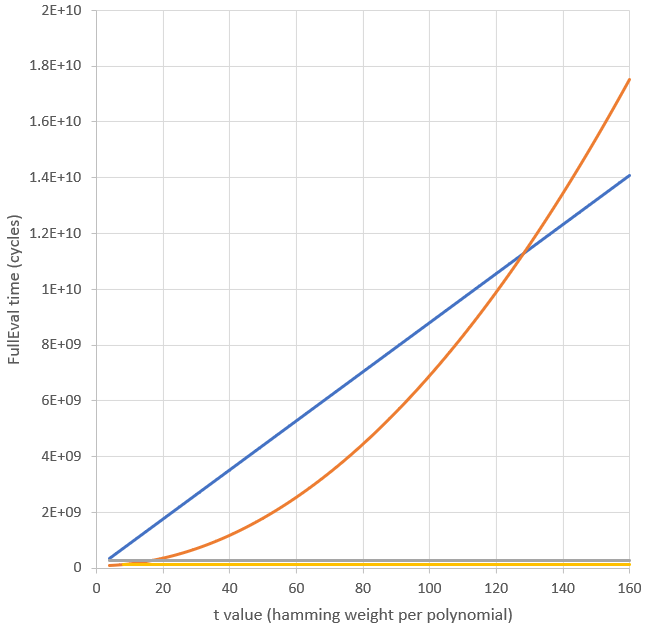
\includegraphics[scale = 0.4]{figures/FullEval_time_PCG.png}
	}
	\subfigure{
		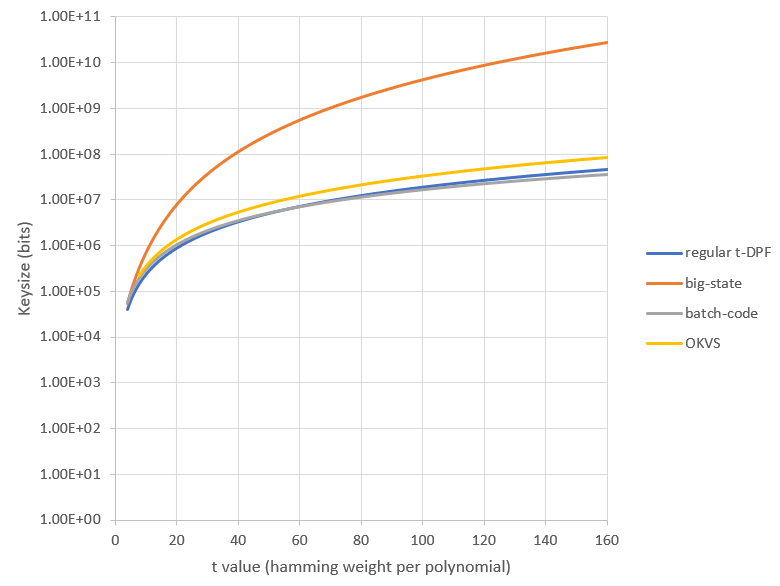
\includegraphics[scale = 0.4]{figures/keysize_PCG.png}
	}
	\caption{Full-domain Evaluation time and keysize of DMPF used in PCG for OLE\cite{cryptoeprint:2022/1035} using four different DMPF constructions. Consider the security parameter $\lambda=128$, the domain size $N = 2^{20}$ and various noise weights per $R$-element, from 4 to 160 (the typical weights per $R$-element in \cite{cryptoeprint:2022/1035} are 5, 16 and 76). To obtain little failure probability, the OKVS-DMPF is only applicable for $t\ge 8$ as considered in \cite{cryptoeprint:2022/320}. PRG evaluation is modeled as two AES evaluations with AES evaluation time $1.3$ cycles per byte. Field multiplications in OKVS-DMPF approach $0.3$ cycles per byte \cite{cryptoeprint:2017/168} for the corresponding field. The actual expand time and seed size of PCG is $\sim \times c^2$ of that the FullEval time and key size of DMPF, where $c$ is the compression factor. }
	\label{fig:detailed_PCG}
\end{figure}

\subsection{PSI-WCA}
plug in new DMPF and analyze advantage interval\\
plug in distributed gen
\subsection{Heavy-hitters}
private heavy-hitter\\
or parallel ORAM?
\section{Acknowledgments}
tbd


\bibliographystyle{ACM-Reference-Format}
\bibliography{references}


%%
%% If your work has an appendix, this is the place to put it.
\appendix
\section{Security Proofs}

\end{document}
\endinput
%%
%% End of file `sample-sigconf.tex'.
